% TikZ and PGF 2.00
% Source: TikZ and PGF manual
\documentclass{article}
\usepackage{tikz}
\usetikzlibrary{shapes,decorations,shadows}
\usetikzlibrary{decorations.pathmorphing}
\usetikzlibrary{decorations.shapes}
\usetikzlibrary{fadings}
\usetikzlibrary{patterns}
\usetikzlibrary{calc}
\usepackage{verbatim}

\begin{comment}
:Title: TikZ and PGF version 2.00
:Slug: pgf-version-2
:Tags: PGF 2.0, Manual
:Grid: 3x3


PGF version 2.0 was released on 2008-02-20 after a few months of hectic activity in CVS and on the `pgf-users`_ mailing list. The new release is packed with new features
and improvements. In this entry I will give a tour of some of the new features. For a full list of changes see the changelog_.

**Note**: Almost all of the examples are from the TikZ and PGF manual. 

.. _pgf-users: http://www.nabble.com/pgf-users-f3583.html
.. _changelog: ftp://cam.ctan.org/tex-archive/graphics/pgf/base/doc/generic/pgf/ChangeLog

Decorations
-----------

Decorations are a new and powerful way of decorating and morphing paths. They are similar to the "snakes" from previous versions of PGF, but much more powerful and general. Here are some of the highlights:

- Arbitrary paths can be decorated, including curves and nodes
- Shapes can be used as decorations
- Decorations can be nested

.. figure:: #pgf2001.png

.. sourcecode:: latex

    % Decorating a node shape
    \usetikzlibrary{decorations.pathmorphing}
    ...
    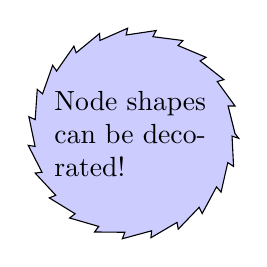
\begin{tikzpicture}
        \node [text width=2cm, decorate, decoration=saw, fill=blue!20,draw,circle]
            {Node shapes can be decorated!};
    \end{tikzpicture}

.. sourcecode:: latex

    % Text decorations
    \usetikzlibrary{decorations.text}
    ...
    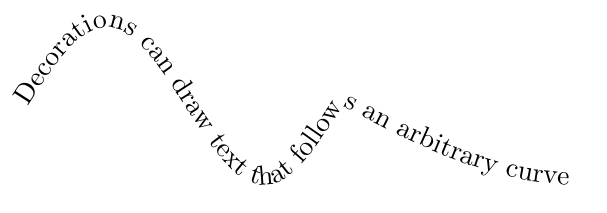
\begin{tikzpicture}
        \path [decorate,decoration={text along path,
            text={Decorations can draw text that follows an arbitrary curve}}]
            (0,0) sin (1,1) cos (2,0) sin (3,-1) cos (4,0) sin (7,-1);
    \end{tikzpicture}

.. sourcecode:: latex

        % Shape decorations
        \usetikzlibrary{decorations.shapes}
        ...
        \tikzset{paint/.style={ draw=#1!50!black, fill=#1!50 },
            decorate with/.style=
            {decorate,decoration={shape backgrounds,shape=#1,shape size=2mm}}}

        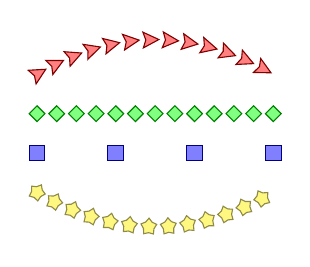
\begin{tikzpicture}
            \draw [decorate with=dart, paint=red] (0,1.5) to[bend left] (3,1.5);
            \draw [decorate with=diamond, paint=green] (0,1) -- (3,1);
            \draw [decorate with=rectangle, paint=blue,
                decoration={shape evenly spread=4}] (0,0.5) -- (3,0.5);
            \draw [decorate with=star, paint=yellow] (0,0) to[bend right] (3,0);
        \end{tikzpicture}

.. sourcecode:: latex

    % Fractal and footprint decorations
    \usetikzlibrary{decorations.fractals}
    \usetikzlibrary{decorations.footprints}
    ...
    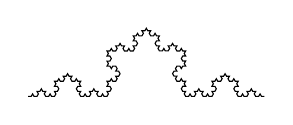
\begin{tikzpicture}[decoration=Koch snowflake]
        \draw decorate{ decorate{ decorate{ decorate{ (0,0) -- (3,0) }}}};
    \end{tikzpicture}

    
\begin{tikzpicture}[decoration={footprints,foot length=10pt,stride length=20pt}]
        \fill decorate{ (0,0) to[bend left] (3.5,0)};
    \end{tikzpicture}


Revamped system for handling options and styles
-----------------------------------------------

PGF has replaced ``xkeyval`` with the new ``pgfkeys`` package. The package provides a powerful key-value management mechanism. A useful new feature is that styles can be parameterized:

.. sourcecode:: latex

    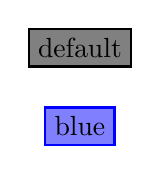
\begin{tikzpicture}[outline/.style={draw=#1,thick,fill=#1!50},
        outline/.default=black]
        \node [outline] at (0,1) {default};
        \node [outline=blue] at (0,0) {blue};
    \end{tikzpicture}

The new style and options system is probably the most notable change from previous version. I highly recommend reading Section 11.4.2 in the manual carefully to get an overview. You can find examples of ``pgfkeys`` usage sprinkled  throughout this entry.

New node shapes
---------------

PGF now ships with an impressive variety of node shapes. Here are a few examples:

.. figure:: #pgf2002.png

.. sourcecode:: latex

    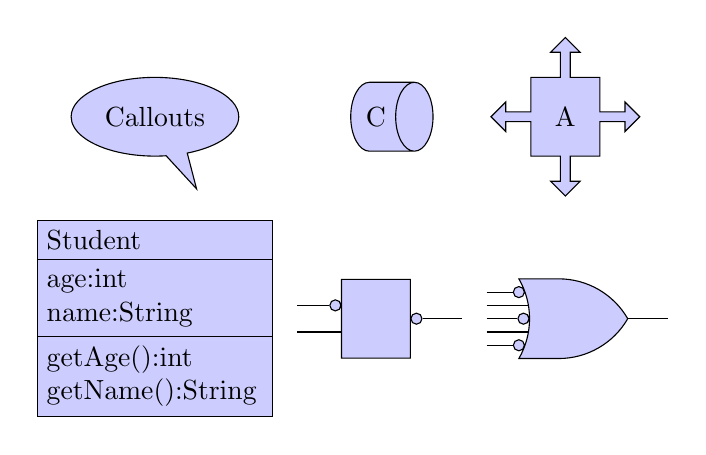
\begin{tikzpicture}
    \matrix[nodes={draw, fill=blue!20},
        row sep=0.3cm,column sep=0.3cm,minimum width=.875cm, minimum height=1cm] {
        \node[ellipse callout] {Callouts}; & \node [cylinder] {C}; &
        %
        \node [arrow box] {A};\\
        %
        \node[rectangle split, rectangle split parts=3, draw, text width=2.75cm]
            {Student
            \nodepart{second}
            age:int \\
            name:String
            \nodepart{third}
            getAge():int \\
            getName():String}; &
        %
        \node[nor gate IEC, draw, logic gate inputs=in] (A) {};
        \draw (A.input 1 -| -1,0) -- (A.input 1) (A.input 2 -| -1,0) -- (A.input 2)
            (A.output) -- ([xshift=0.5cm]A.output); &
        %
        \node[or gate US, draw,logic gate inputs=inini] (A) {};
        \foreach \a in {1,...,5}
            \draw (A.input \a -| -1,0) -- (A.input \a);
            \draw (A.output) -- ([xshift=0.5cm]A.output);\\
    };
    \end{tikzpicture}

See Chapter 39 in the manual for a complete list of node shapes. Of special interest are the logic gate and multipart shapes.

Fitting library
---------------

Defines a convenient ``fit`` option for creating a node that is sized to exactly fit a set of coordinates.

.. figure:: #pgf2003.png

.. sourcecode:: latex

    \usetikzlibrary{fit}
    ...
    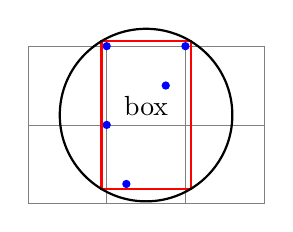
\begin{tikzpicture}[inner sep=0pt,thick,
        dot/.style={fill=blue,circle,minimum size=3pt}]
        \draw[help lines] (0,0) grid (3,2);
        \node[dot] (a) at (1,1) {};
        \node[dot] (b) at (2,2) {};
        \node[dot] (c) at (1,2) {};
        \node[dot] (d) at (1.25,0.25) {};
        \node[dot] (e) at (1.75,1.5) {};
        \node[draw=red, fit=(a) (b) (c) (d) (e)] {box};
        \node[draw,circle,fit=(a) (b) (c) (d) (e)] {};
    \end{tikzpicture}




Shadows
-------

The shadow library can apply shadows to paths and node shapes:

.. figure:: extra/shadowlibrary.png

.. sourcecode:: latex

    \usetikzlibary{shadows}
    ...
    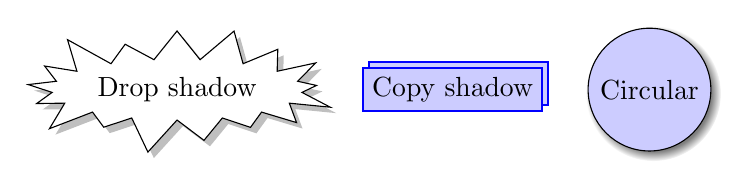
\begin{tikzpicture}
        \node[starburst,drop shadow,fill=white,draw] {Drop shadow};
        \node[copy shadow,fill=blue!20,draw=blue,thick] at (3.5,0) {Copy shadow};
        \node[circle,circular drop shadow,fill=blue!20,draw] at (6,0) {Circular};
    \end{tikzpicture}




More options for node positioning
---------------------------------

New and more convenient placements options are now available if you load the ``positioning`` library. Here are a few examples:

.. figure:: #pgf2007.png

.. sourcecode:: latex

    \usetikzlibrary{positioning}
    ...
    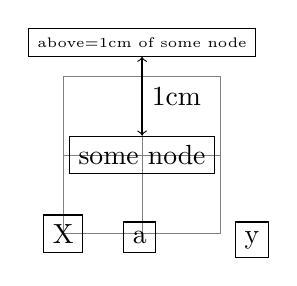
\begin{tikzpicture}[every node/.style=draw]
        \draw[help lines] (0,0) grid (2,2);
        \node (some node) at (1,1) {some node};
        \node (other node) [above=1cm of some node] {\tiny above=1cm of some node};
        \draw [<->] (some node) -- (other node)
        node [midway,right,draw=none] {1cm};

        \node (X) at (0,0) {X};
        \node (a) [base right=0.5cm of X ] {a};
        \node (y) [base right=of a] {y};
    \end{tikzpicture}

See Chapter 15.5.3 for more details. Another useful addition is the ``chains`` library:

.. figure:: #pgf2005.png

.. sourcecode:: latex

    \usetikzlibrary{chains}
    ...
    \begin{tikzpicture}[every on chain/.style=join,every join/.style=->,
        node distance=2mm and 1cm]
        { [start chain=trunk]
            \node [on chain] {A};
            \node [on chain] {B};
            { [start branch=numbers going below] } % just a declaration,
            { [start branch=greek going above] } % we will come back later
            \node [on chain] {C};
            % Now come the branches...
            { [continue branch=numbers]
                \node [on chain] {1};
                \node [on chain] {2};
            }
            { [continue branch=greek]
                \node [on chain] {$\alpha$};
                \node [on chain] {$\beta$};
            }
        }
    \end{tikzpicture}

Coordinate calculations
-----------------------

It is now possible to do some basic calculations on coordinates. The allowed operations are addition, subtraction, scaling, midpoint calculations and projection. To use coordinate calculations you need to load the ``calc library``. Here are a few examples:

.. figure:: #pgf2008.png

.. sourcecode:: latex

    \usetikzlibrary{calc}

    ...
    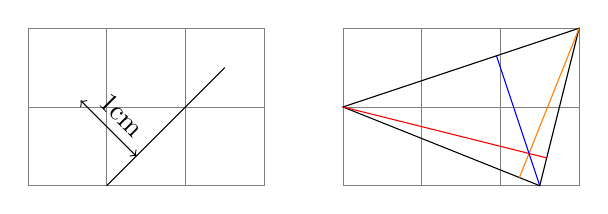
\begin{tikzpicture}
        \begin{scope}
            \draw [help lines] (0,0) grid (3,2);
            \coordinate (a) at (1,0);
            \coordinate (b) at ($(a)+1/2*(3,3)$);
            \draw (a) -- (b);
            \coordinate (c) at ($ (a)!.25!(b) $);
            \coordinate (d) at ($ (c)!1cm!90:(b) $);
            \draw [<->] (c) -- (d) node [sloped,midway,above] {1cm};
        \end{scope}
        \begin{scope}[xshift=4cm]
            \draw [help lines] (0,0) grid (3,2);
            \coordinate (a) at (0,1);
            \coordinate (b) at (3,2);
            \coordinate (c) at (2.5,0);
            \draw (a) -- (b) -- (c) -- cycle;
            \draw[red] (a) -- ($(b)!(a)!(c)$);
            \draw[orange] (b) -- ($(a)!(b)!(c)$);
            \draw[blue] (c) -- ($(a)!(c)!(b)$);
        \end{scope}
    \end{tikzpicture}

Coordinate calculations are described in Chapter 12.4 in the manual.

Preactions and postactions
--------------------------

Allows you to manipulate a path before and after it is drawn:

.. figure:: #pgf2009.png

.. sourcecode:: latex

    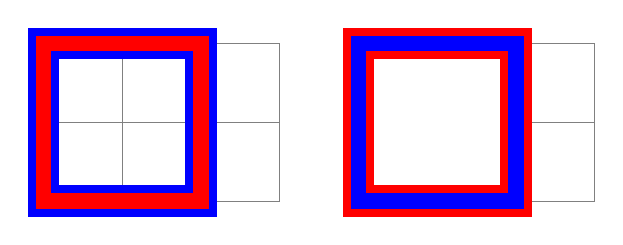
\begin{tikzpicture}
        { []
            \draw[help lines] (0,0) grid (3,2);
            \draw
                [preaction={draw,line width=4mm,blue}]
                [line width=2mm,red] (0,0) rectangle (2,2);
        }
        { [xshift=4cm]

            \draw[help lines] (0,0) grid (3,2);
            \draw
                [postaction={draw,line width=2mm,blue}]
                [line width=4mm,red,fill=white] (0,0) rectangle (2,2);
        }
    \end{tikzpicture}

See Chapter 14.8 in the manual for more details.


Other changes
-------------

The ``\foreach`` command now allows a macro name to be given as a list argument:

.. sourcecode:: latex

    \newcommand\mylist{1/a,2/b,3/c,4/d}
    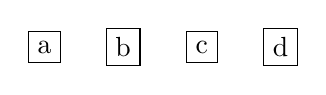
\begin{tikzpicture}
        \foreach \x/\lbl in \mylist {
            \node[draw] at (\x,0) {\lbl};
        }
    \end{tikzpicture}

Coordinates like ``(2,3cm)`` are now allowed. Has the same effect as:

.. sourcecode:: latex

    ([shift={(2,0)}]0pt,3cm)

*Improved support for transparency*. TikZ now support fadings and transparency groups:

.. figure:: extra/trgroupfadings.png

.. sourcecode:: latex

    \usetikzlibrary{patterns}
    ...
    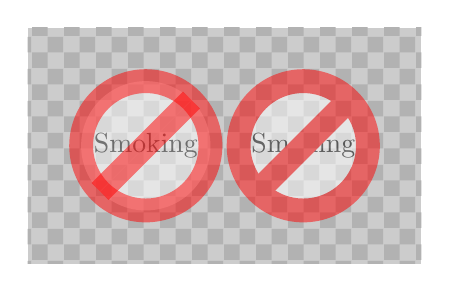
\begin{tikzpicture}
        % Checker board
        \fill [black!20] (-1.5,-1.5) rectangle (3.5,1.5);
        \pattern [pattern=checkerboard,pattern color=black!30]
        (-1.5,-1.5) rectangle (3.5,1.5);
        \node at (0,0) [opacity=0.5,forbidden sign,line width=2ex,
            draw=red,fill=white] {Smoking};
        \begin{scope}[opacity=.5,transparency group]
            \node at (2,0) [forbidden sign,line width=2ex,draw=red,fill=white]
            {Smoking};
        \end{scope}
    \end{tikzpicture}

.. sourcecode:: latex

    \usetikzlibrary{patterns,fadings}
    ...
    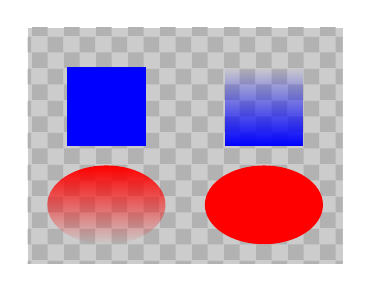
\begin{tikzpicture}[path fading=south]
        % Checker board
        \fill [black!20] (0,0) rectangle (4,3);
        \pattern [pattern=checkerboard,pattern color=black!30]
            (0,0) rectangle (4,3);
        \fill [color=blue] (0.5,1.5) rectangle +(1,1);
        \fill [color=blue,path fading=north] (2.5,1.5) rectangle +(1,1);
        \fill [color=red,path fading] (1,0.75) ellipse (.75 and .5);
        \fill [color=red] (3,0.75) ellipse (.75 and .5);
    \end{tikzpicture}

*Shorthand for scope environments*. The ``scopes`` library defines a shorthand notation for starting and ending scope environments. It allows you to start and end a scope using braces provided the opening brace is followed by options in square brackets:

.. sourcecode:: latex

    \usetikzlibrary{scopes}
    ...
    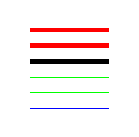
\begin{tikzpicture}
        { [ultra thick]
            { [red]
                \draw (0mm,10mm) -- (10mm,10mm);
                \draw (0mm,8mm) -- (10mm,8mm);
            }
            \draw (0mm,6mm) -- (10mm,6mm);
        }
        { [green]
            \draw (0mm,4mm) -- (10mm,4mm);
            \draw (0mm,2mm) -- (10mm,2mm);
            \draw[blue] (0mm,0mm) -- (10mm,0mm);
        }
    \end{tikzpicture}

*New transformations*. The transformation options ``transform canvas`` and ``scale around`` have been added. Described in Chapter 21.4 and 21.3 respectively.



:Source: The PGF and TikZ manual



\end{comment}


\usetikzlibrary{decorations.text}
\usetikzlibrary{decorations.footprints}
\usetikzlibrary{decorations.fractals}
\usetikzlibrary{shapes.gates.logic.IEC}
\usetikzlibrary{shapes.gates.logic.US}
\usetikzlibrary{fit,chains}
\usetikzlibrary{positioning}
\usepgflibrary{shapes}
\usetikzlibrary{scopes}


\begin{document}


\tikzset{paint/.style={ draw=#1!50!black, fill=#1!50 },
    decorate with/.style=
    {decorate,decoration={shape backgrounds,shape=#1,shape size=2mm}}}

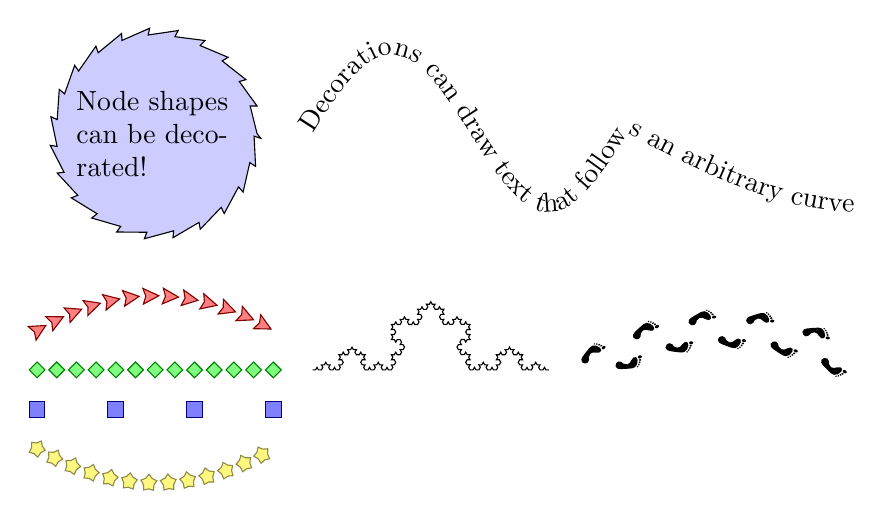
\begin{tikzpicture}
\node [text width=2cm, decorate, decoration=saw, fill=blue!20,draw,circle]
    {Node shapes can be decorated!};
{ [xshift=2cm]
    \path [decorate,decoration={text along path,
            text={Decorations can draw text that follows an arbitrary curve}}]
            (0,0) sin (1,1) cos (2,0) sin (3,-1) cos (4,0) sin (7,-1);
}
%
{[xshift=-1.5cm,yshift=-4cm]
    \draw [decorate with=dart, paint=red] (0,1.5) to[bend left] (3,1.5);
    \draw [decorate with=diamond, paint=green] (0,1) -- (3,1);
    \draw [decorate with=rectangle, paint=blue,
        decoration={shape evenly spread=4}] (0,0.5) -- (3,0.5);
    \draw [decorate with=star, paint=yellow] (0,0) to[bend right] (3,0);
}
%
{ [xshift=2cm,yshift=-3cm,
    decoration=Koch snowflake]
    \draw decorate{ decorate{ decorate{ decorate{ (0,0) -- (3,0) }}}};
}
%
{[xshift=5.5cm,yshift=-3cm,
    decoration={footprints,foot length=10pt,stride length=20pt}]
    \fill decorate{ (0,0) to[bend left] (3.5,0)};
}
\end{tikzpicture}


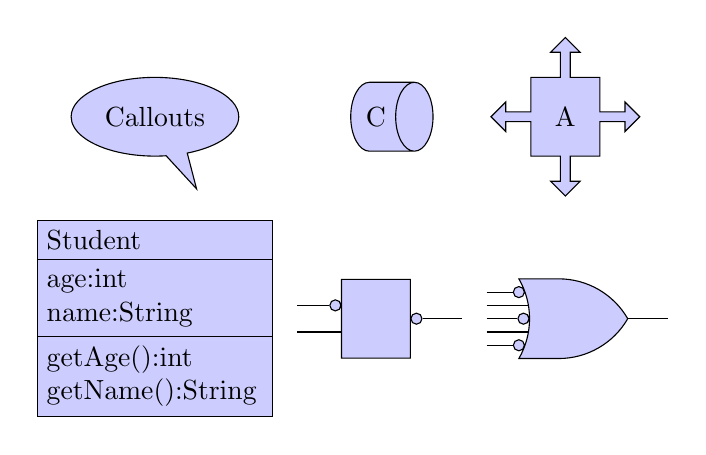
\begin{tikzpicture}
\matrix[nodes={draw, fill=blue!20},
    row sep=0.3cm,column sep=0.3cm,minimum width=.875cm, minimum height=1cm] {
    \node[ellipse callout] {Callouts}; & \node [cylinder] {C}; &
    %
    \node [arrow box] {A};\\
    %
    \node[rectangle split, rectangle split parts=3, draw, text width=2.75cm]
        {Student
        \nodepart{second}
        age:int \\
        name:String
        \nodepart{third}
        getAge():int \\
        getName():String}; &
    %
    \node[nor gate IEC, draw, logic gate inputs=in] (A) {};
    \draw (A.input 1 -| -1,0) -- (A.input 1) (A.input 2 -| -1,0) -- (A.input 2)
        (A.output) -- ([xshift=0.5cm]A.output); &
    %
    \node[or gate US, draw,logic gate inputs=inini] (A) {};
    \foreach \a in {1,...,5}
        \draw (A.input \a -| -1,0) -- (A.input \a);
        \draw (A.output) -- ([xshift=0.5cm]A.output);\\
};
\end{tikzpicture}

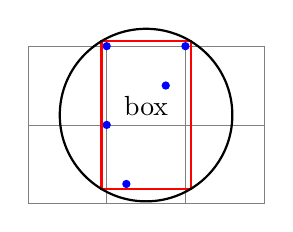
\begin{tikzpicture}[inner sep=0pt,thick,
    dot/.style={fill=blue,circle,minimum size=3pt}]
    \draw[help lines] (0,0) grid (3,2);
    \node[dot] (a) at (1,1) {};
    \node[dot] (b) at (2,2) {};
    \node[dot] (c) at (1,2) {};
    \node[dot] (d) at (1.25,0.25) {};
    \node[dot] (e) at (1.75,1.5) {};
    \node[draw=red, fit=(a) (b) (c) (d) (e)] {box};
    \node[draw,circle,fit=(a) (b) (c) (d) (e)] {};
\end{tikzpicture}

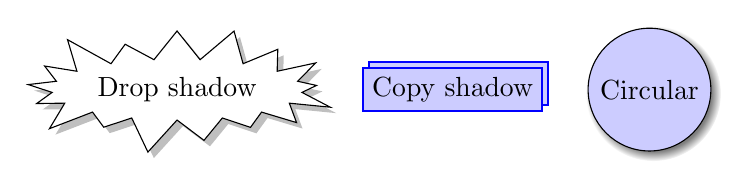
\begin{tikzpicture}
    \node[starburst,drop shadow,fill=white,draw] {Drop shadow};
    \node[copy shadow,fill=blue!20,draw=blue,thick] at (3.5,0) {Copy shadow};
    \node[circle,circular drop shadow,fill=blue!20,draw] at (6,0) {Circular};
\end{tikzpicture}

\begin{tikzpicture}[every on chain/.style=join,every join/.style=->,
    node distance=2mm and 1cm]
    { [start chain=trunk]
        \node [on chain] {A};
        \node [on chain] {B};
        { [start branch=numbers going below] } % just a declaration,
        { [start branch=greek going above] } % we will come back later
        \node [on chain] {C};
        % Now come the branches...
        { [continue branch=numbers]
            \node [on chain] {1};
            \node [on chain] {2};
        }
        { [continue branch=greek]
            \node [on chain] {$\alpha$};
            \node [on chain] {$\beta$};
        }
    }
\end{tikzpicture}

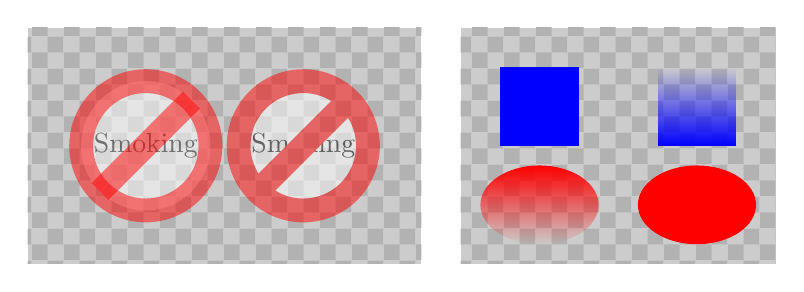
\begin{tikzpicture}
    % Checker board
    \fill [black!20] (-1.5,-1.5) rectangle (3.5,1.5);
    \pattern [pattern=checkerboard,pattern color=black!30]
        (-1.5,-1.5) rectangle (3.5,1.5);
    \node at (0,0) [opacity=0.5,forbidden sign,line width=2ex,
        draw=red,fill=white]
        {Smoking};
    \begin{scope}[opacity=.5,transparency group]
        \node at (2,0) [forbidden sign,line width=2ex,draw=red,fill=white]
        {Smoking};
    \end{scope}
    \begin{scope}[xshift=4cm,yshift=-1.5cm,path fading=south]
        % Checker board
        \fill [black!20] (0,0) rectangle (4,3);
        \pattern [pattern=checkerboard,pattern color=black!30]
            (0,0) rectangle (4,3);
        \fill [color=blue] (0.5,1.5) rectangle +(1,1);
        \fill [color=blue,path fading=north] (2.5,1.5) rectangle +(1,1);
        \fill [color=red,path fading] (1,0.75) ellipse (.75 and .5);
        \fill [color=red] (3,0.75) ellipse (.75 and .5);
    \end{scope}
\end{tikzpicture}

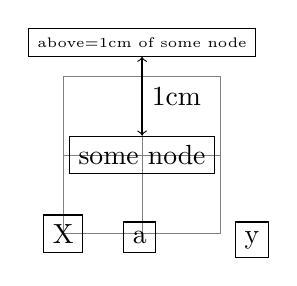
\begin{tikzpicture}[every node/.style=draw]
    \draw[help lines] (0,0) grid (2,2);
    \node (some node) at (1,1) {some node};
    \node (other node) [above=1cm of some node] {\tiny above=1cm of some node};
    \draw [<->] (some node) -- (other node)
    node [midway,right,draw=none] {1cm};

    \node (X) at (0,0) {X};
    \node (a) [base right=0.5cm of X ] {a};
    \node (y) [base right=of a] {y};
\end{tikzpicture}

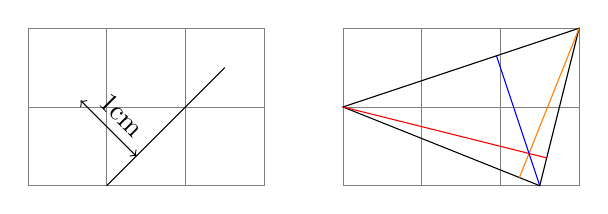
\begin{tikzpicture}
    { []
        \draw [help lines] (0,0) grid (3,2);
        \coordinate (a) at (1,0);
        \coordinate (b) at ($(a)+1/2*(3,3)$);
        \draw (a) -- (b);
        \coordinate (c) at ($ (a)!.25!(b) $);
        \coordinate (d) at ($ (c)!1cm!90:(b) $);
        \draw [<->] (c) -- (d) node [sloped,midway,above] {1cm};
    }
    { [xshift=4cm]
        \draw [help lines] (0,0) grid (3,2);
        \coordinate (a) at (0,1);
        \coordinate (b) at (3,2);
        \coordinate (c) at (2.5,0);
        \draw (a) -- (b) -- (c) -- cycle;
        \draw[red] (a) -- ($(b)!(a)!(c)$);
        \draw[orange] (b) -- ($(a)!(b)!(c)$);
        \draw[blue] (c) -- ($(a)!(c)!(b)$);
    }
\end{tikzpicture}


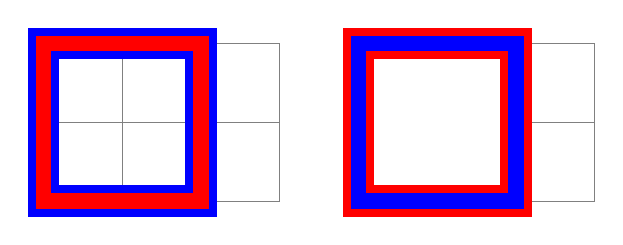
\begin{tikzpicture}
    { []
        \draw[help lines] (0,0) grid (3,2);
        \draw
            [preaction={draw,line width=4mm,blue}]
            [line width=2mm,red] (0,0) rectangle (2,2);
    }
    { [xshift=4cm]

        \draw[help lines] (0,0) grid (3,2);
        \draw
            [postaction={draw,line width=2mm,blue}]
            [line width=4mm,red,fill=white] (0,0) rectangle (2,2);
    }
\end{tikzpicture}


\end{document}
